\chapter{随机优化、动量与非凸收敛}
\label{l3:chapter}

\begin{coursebox}{学习目标与课时安排}
本讲安排为两个理论学时和一个实验学时。理论第一部分回答：随机梯度在什么意义下正确，批量大小如何进入稳定性和误差；第二部分回答：动量何时加速，非凸问题究竟能够保证什么。实验用可精确求解的一维随机回归核对理论，再把记录方法迁移到神经网络训练。

核心内容是条件无偏性、高斯回归的均方递推、非凸一阶平稳性界和 Heavy Ball 的稳定区间。有限总体抽样证明、矩阵稳态协方差、局部临界批量模型以及 Nesterov 的完整加速理论列为选读。学完本讲，应能在报告中分别说明“均值下降”“均方稳定”“梯度变小”和“验证集性能改善”，并知道这些结论需要不同证据。
\end{coursebox}

\section{随机梯度的对象与条件}
\label{l3:stochastic-model}

前两讲把目标函数和梯度视为可精确计算的对象。训练神经网络时，完整数据集上的一次梯度可能很昂贵，因此每一步只使用一个批次。随机性带来了计算节省，也改变了我们能够提出的收敛问题：一条轨迹可能上下波动，期望损失可能下降，参数方差却未必消失。分析必须先说明期望对什么随机量取值。

有两类常用目标。对固定训练集，经验风险为
\begin{equation}
 F(w)=\frac{1}{N}\sum_{i=1}^{N}f_i(w),\qquad w\in\R^d.
 \label{l3:finite-sum}
\end{equation}
对不断取得的新样本，人口风险为
\begin{equation}
 F(w)=\E_z[\ell(w;z)].
 \label{l3:population}
\end{equation}
在可交换微分与期望的条件下，后者满足
$\nabla F(w)=\E_z[\nabla_w\ell(w;z)]$。这项可交换性是模型假设的一部分，不是由“取平均”自动得到的。以下有限和模型不需要该项分析条件。

令 $\mathcal F_t$ 表示第 $t$ 次取样之前的全部信息，包括 $w_t$、过去的批次和优化器状态。我们用 $g_t$ 表示本次随机梯度，并写出迭代
\begin{equation}
 w_{t+1}=w_t-\eta_t g_t.
 \label{l3:sgd}
\end{equation}
最常用的假设不是无条件的 $\E[g_t]=\nabla F(w_t)$；右边本身仍是随机量。正确写法是
\begin{equation}
 \E[g_t\mid\mathcal F_t]=\nabla F(w_t),\qquad
 \E[\norm{g_t-\nabla F(w_t)}^2\mid\mathcal F_t]\leq\frac{\sigma^2}{B}.
 \label{l3:unbiased-variance}
\end{equation}
第一式说明，在已经知道当前参数的条件下，本次估计没有系统偏差；第二式另外限制了噪声强度。无偏性不蕴含方差有界，方差有界也不蕴含无偏性。

\subsection{为什么会出现 $1/B$}

固定一个参数 $w$，设独立样本梯度 $h_1,\ldots,h_B$ 的均值为 $\bar g=\nabla F(w)$，协方差为 $\Sigma(w)$。对于平均梯度
\[
 g_B=\frac1B\sum_{b=1}^{B}h_b,
\]
独立性使交叉协方差为零，因此
\begin{equation}
 \E[g_B]=\bar g,\qquad
 \Cov(g_B)=\frac{\Sigma(w)}{B},\qquad
 \E\norm{g_B-\bar g}^2=\frac{\tr\Sigma(w)}{B}.
 \label{l3:batch-variance}
\end{equation}
这一等式适用于独立取样或固定数据集上的有放回均匀抽样。真实批次如果包含相邻时间点、同一序列的 token，或强相关的增强视图，就应从
\begin{equation}
 \Cov(g_B)=\frac1{B^2}\sum_{b=1}^{B}\sum_{c=1}^{B}\Cov(h_b,h_c)
 \label{l3:correlated-batch}
\end{equation}
开始。批次中样本数量加倍，未必使方差减半；需要查看非对角项。

\begin{proposition}[不放回批次的有限总体修正，选读]
固定 $w$，令 $h_i=\nabla f_i(w)$，$\bar h=N^{-1}\sum_i h_i$，并采用分母为 $N$ 的总体协方差
\[
 \Sigma_N=\frac1N\sum_{i=1}^{N}(h_i-\bar h)(h_i-\bar h)^\top.
\]
若从 $N>1$ 个样本中均匀不放回抽取 $B$ 个，则
\begin{equation}
 \Cov(g_B)=\frac{N-B}{B(N-1)}\Sigma_N.
 \label{l3:finite-population}
\end{equation}
\end{proposition}
\begin{proof}
令 $u_i=h_i-\bar h$，则 $\sum_i u_i=0$。一个被抽中的位置的二阶矩为 $\Sigma_N$；两个不同位置的交叉矩为
\[
 \frac{1}{N(N-1)}\sum_{i\ne j}u_i u_j^\top
 =-\frac{\Sigma_N}{N-1}.
\]
把 $B$ 个对角项和 $B(B-1)$ 个交叉项代入平均值的协方差，即得结论。
\end{proof}

这里是“在固定 $w$ 处重新抽一个均匀批次”的计算。一个 epoch 内打乱数据后逐批使用时，当前参数已依赖前面见过的样本，剩余样本的条件分布有所改变，因此不能不加说明地套用式\eqref{l3:unbiased-variance}。随机重排有专门的分析；本讲的证明先使用每步独立抽样模型。此外，$B=N$ 消除了固定训练集上的批次噪声，但并未消除训练集相对真实分布的统计误差。

\section{一个可以完全算清楚的随机回归模型}
\label{l3:gaussian-regression}

\subsection{数据、目标与随机梯度}

考虑一维模型 $\hat y=ax$。真实数据由
\begin{equation}
 x\sim\mathcal N(0,s^2),\qquad y=a_\star x+\varepsilon,
 \qquad \E\varepsilon=0,\quad \Var(\varepsilon)=\tau^2
 \label{l3:gaussian-data}
\end{equation}
生成，其中 $s^2>0$，$\varepsilon$ 与 $x$ 独立，不同样本和不同步之间也独立。损失为 $\ell(a;x,y)=\tfrac12(ax-y)^2$。记误差 $e=a-a_\star$，人口风险是
\begin{equation}
 F(a)=\frac{s^2}{2}e^2+\frac{\tau^2}{2},\qquad
 F(a)-F(a_\star)=\frac{s^2}{2}e^2.
 \label{l3:regression-risk}
\end{equation}
后面讨论的是超额风险，不能把不可约的 $\tau^2/2$ 也解释为优化误差。

在第 $t$ 步用 $B$ 个新样本，定义
\[
 A_t=\frac1B\sum_{b=1}^{B}x_{t,b}^2,
 \qquad b_t=\frac1B\sum_{b=1}^{B}x_{t,b}\varepsilon_{t,b}.
\]
批次梯度和参数误差更新恰好是
\begin{equation}
 g_t=A_t e_t-b_t,\qquad
 e_{t+1}=(1-\eta A_t)e_t+\eta b_t.
 \label{l3:random-coefficient}
\end{equation}
这不是“固定曲率加一个常方差扰动”的模型。随机批次同时改变曲率 $A_t$，因此包含乘性噪声。正是这一项使均值稳定与均方稳定出现差异。

高斯四阶矩 $\E[x^4]=3s^4$ 给出
\begin{align}
 \E A_t&=s^2,&
 \E A_t^2&=s^4\left(1+\frac2B\right),\label{l3:A-moments}\\
 \E b_t&=0,&
 \E b_t^2&=\frac{s^2\tau^2}{B},&
 \E[A_t b_t]&=0.\label{l3:b-moments}
\end{align}
例如最后一个等式可以先对所有 $x_{t,b}$ 条件化，再利用每个噪声 $\varepsilon_{t,b}$ 的零均值得到。它不要求标签噪声本身为高斯。

\subsection{均值收敛不是均方收敛}

令 $m_t=\E e_t$、$q_t=\E e_t^2$。由于新批次独立于 $e_t$，对式\eqref{l3:random-coefficient}取期望得到
\begin{equation}
 m_{t+1}=(1-\eta s^2)m_t.
 \label{l3:mean-recurrence}
\end{equation}
平方后再取期望，使用式\eqref{l3:A-moments}--\eqref{l3:b-moments}，得到精确递推
\begin{equation}
 \boxed{q_{t+1}=r_B(\eta)q_t+\frac{\eta^2s^2\tau^2}{B}},
 \qquad
 r_B(\eta)=(1-\eta s^2)^2+\frac{2\eta^2s^4}{B}.
 \label{l3:mean-square-recurrence}
\end{equation}
注意 $q_t$ 是关于最优参数的二阶矩，包含均值平方和方差；一般不等于 $\Var(a_t)$。

\begin{theorem}[高斯随机回归的稳定条件]
在式\eqref{l3:gaussian-data}的假设下，取常步长 $\eta>0$，并假设初始误差有有限二阶矩。
均值递推的渐近稳定条件是
\begin{equation}
 0<\eta s^2<2.
 \label{l3:mean-stability}
\end{equation}
均方递推的收缩条件是
\begin{equation}
 \boxed{0<\eta s^2<\frac{2B}{B+2}}.
 \label{l3:mean-square-stability}
\end{equation}
在后一条件下，
\begin{align}
 q_t&=r_B(\eta)^t q_0+
 \frac{\eta^2s^2\tau^2}{B}\frac{1-r_B(\eta)^t}{1-r_B(\eta)},\label{l3:finite-time-q}\\
 q_\infty&=\frac{\eta\tau^2}{B\left[2-\eta s^2(1+2/B)\right]}.
 \label{l3:gaussian-floor}
\end{align}
\end{theorem}
\begin{proof}
均值的结论来自 $|1-\eta s^2|<1$。令 $h=\eta s^2>0$，均方系数小于一等价于
\[
 1-2h+h^2\left(1+\frac2B\right)<1,
\]
即 $h<2/(1+2/B)$。在 $r_B<1$ 时对仿射递推求几何级数，并化简常数项，得到其余两式。
\end{proof}

当 $\tau^2>0$ 且 $r_B=1$ 时，二阶矩线性增长；$r_B>1$ 时通常指数增长。若 $\tau^2=0$，则 $q_t=r_B^tq_0$；边界处二阶矩保持而不收缩。初值恰好为最优点且没有标签噪声是一个退化例外，不能据此改变稳定区间的定义。

\begin{example}[均值一步到零，均方却发散]
取 $s^2=1$、$B=1$、$\eta=1$、$\tau^2=1/4$，并令 $e_0=1$。式\eqref{l3:mean-recurrence}给出 $m_t=0$ 对所有 $t\geq1$ 成立。可是
\[
 q_{t+1}=2q_t+\frac14,
 \qquad q_t=\frac54\,2^t-\frac14.
\]
因此平均参数恰好等于 $a_\star$，平均超额风险却不断增大。原因是不同轨迹的正负误差可以在一阶矩中抵消，而平方不能抵消。只画多次运行的平均参数，会把一个均方不稳定算法误读为快速收敛。

这个例子还提醒我们注意蒙特卡洛估计：乘性噪声可使少量大误差轨迹显著影响二阶矩，有限重复次数得到的曲线不一定贴合理论值。实验应报告重复次数，并同时查看误差分布，而不能把一条平滑曲线当作证明。
\end{example}

\subsection{这里的噪声方差并不是全局常数}

条件于当前误差，有
\begin{equation}
 \Var(g_t\mid e_t)=\frac{2s^4e_t^2+s^2\tau^2}{B}.
 \label{l3:state-dependent-noise}
\end{equation}
误差很大时，梯度估计本身也更不稳定。这个模型满足无偏性，但不满足在整个实数轴上以同一个 $\sigma^2$ 控制条件方差的假设。后面使用有界方差的非凸定理时，必须重新核对假设；不能因为两个结果都涉及 SGD，就把结论直接拼在一起。如果只在一个有界区域内分析，或另外证明迭代二阶矩受控，才有可能得到适用的局部或期望型界。

\section{加性噪声模型与稳态误差}
\label{l3:additive-noise}

为分离曲率和噪声的作用，再看一个更简单但不同的模型：
\begin{equation}
 F(e)=\frac\lambda2e^2,
 \qquad g_t=\lambda e_t+\xi_t,
 \qquad \E[\xi_t\mid\mathcal F_t]=0,
 \qquad \E[\xi_t^2\mid\mathcal F_t]=\frac{\sigma_g^2}{B},
 \label{l3:additive-model}
\end{equation}
其中 $\lambda>0$。现在随机性不改变曲率，误差递推为
\[
 e_{t+1}=(1-\eta\lambda)e_t-\eta\xi_t.
\]
在 $0<\eta\lambda<2$ 下，其稳态二阶矩与超额损失为
\begin{equation}
 \E e_\infty^2=
 \frac{\eta\sigma_g^2}{B\lambda(2-\eta\lambda)},
 \qquad
 \boxed{\E F(e_\infty)=
 \frac{\eta\sigma_g^2}{2B(2-\eta\lambda)}}.
 \label{l3:additive-floor}
\end{equation}
当 $\eta\lambda\ll1$，损失近似为 $\eta\sigma_g^2/(4B)$。因此小步长下常说的“噪声地板正比于 $\eta/B$”有一个清楚的适用范围：固定曲率、指定的梯度噪声模型以及远离稳定边界的步长。接近边界时，分母不能忽略。

\begin{remark}[矩阵版本，选读]
设 $F(e)=\tfrac12e^\top He$，$H\succ0$，并将本节的加性噪声假设推广为 $\E[\xi_t\mid\mathcal F_t]=0$、$\E[\xi_t\xi_t^\top\mid\mathcal F_t]=\Sigma/B$。假设初始误差具有有限二阶矩，且 $0<\eta<2/\lambda_{\max}(H)$。此时均值趋零，协方差极限 $C$ 满足离散 Lyapunov 方程
\begin{equation}
 C=(I-\eta H)C(I-\eta H)+\frac{\eta^2}{B}\Sigma.
 \label{l3:lyapunov}
\end{equation}
当 $\eta\norm{H}_2$ 很小时，一阶近似为
$HC+CH\approx\eta\Sigma/B$。取迹得到
\[
 \E F(e)=\frac12\tr(HC)\approx\frac{\eta}{4B}\tr\Sigma.
\]
这是对稳态损失的近似，不是对参数协方差的近似；后者仍明显依赖曲率方向。特别地，不能把这个损失公式写成 $\eta\tr(H\Sigma)/(2B)$。
\end{remark}

\begin{example}[批量扩大四倍，学习率也扩大四倍]
回到精确高斯回归模型，取 $s^2=\tau^2=1$。比较 $(B,\eta)=(4,0.2)$ 与 $(16,0.8)$，两者均满足均方稳定条件。式\eqref{l3:gaussian-floor}给出
\[
 q_\infty^{(4)}=\frac{0.2}{4(2-0.3)}\approx0.02941,
 \qquad
 q_\infty^{(16)}=\frac{0.8}{16(2-0.9)}\approx0.04545.
\]
两者的 $\eta/B$ 相同，稳态误差却不相同。小步长近似把二者都预测为 $\eta/(2B)=0.025$；第二组更接近稳定边界，近似误差更大。

更大的批次每一步使用更多样本。若固定总样本预算，第二组只能执行第一组四分之一的步数。因此比较“同样训练步数的损失”与“同样样本预算的损失”是两个不同实验。本例既不证明大批次差，也不证明线性缩放没有价值；它准确指出了缩放规则不能脱离稳定分母和资源口径。
\end{example}

\section{非凸问题：保证的是一阶平稳性}
\label{l3:nonconvex}

深度网络的目标通常不是凸函数。我们仍可使用第一讲的下降引理，但终点从函数值差改为梯度范数。下面的结论是理解非凸 SGD 的基本模板，其研究背景可参见\citet{Ghadimi2013}。

\begin{theorem}[常步长非凸 SGD 的平均梯度界]
假设 $F:\R^d\to\R$ 可微、梯度为 $L$-Lipschitz，并有有限下界 $F_{\inf}$。假设式\eqref{l3:unbiased-variance}对每一步成立，且相关随机变量有使下述期望存在的有限矩。令 $w_0$ 固定，使用常步长 $0<\eta\leq1/L$，并记 $\Delta=F(w_0)-F_{\inf}$。则
\begin{equation}
 \boxed{\frac1T\sum_{t=0}^{T-1}\E\norm{\nabla F(w_t)}^2
 \leq\frac{2\Delta}{\eta T}+\frac{L\eta\sigma^2}{B}}.
 \label{l3:stationarity-bound}
\end{equation}
若 $R$ 独立、均匀取自 $\{0,\ldots,T-1\}$，左侧也等于
$\E\norm{\nabla F(w_R)}^2$。
\end{theorem}
\begin{proof}
由光滑性和更新式，
\[
 F(w_{t+1})\leq F(w_t)-\eta\inner{\nabla F(w_t)}{g_t}
 +\frac{L\eta^2}{2}\norm{g_t}^2.
\]
条件无偏性给出
\[
 \E[\norm{g_t}^2\mid\mathcal F_t]
 =\norm{\nabla F(w_t)}^2+
 \E[\norm{g_t-\nabla F(w_t)}^2\mid\mathcal F_t].
\]
因此
\begin{align}
 \E[F(w_{t+1})\mid\mathcal F_t]
 &\leq F(w_t)-\eta\left(1-\frac{L\eta}{2}\right)
 \norm{\nabla F(w_t)}^2+\frac{L\eta^2\sigma^2}{2B}\notag\\
 &\leq F(w_t)-\frac\eta2\norm{\nabla F(w_t)}^2
 +\frac{L\eta^2\sigma^2}{2B}.
 \label{l3:conditional-descent}
\end{align}
再取全期望，从 $t=0$ 累加到 $T-1$，利用望远镜求和与
$\E F(w_T)\geq F_{\inf}$，即可得到结论。关于 $w_R$ 的说法来自对均匀随机下标取期望。
\end{proof}

\subsection{怎样读这个上界}

第一项是有限时间的优化误差，偏好较大步长；第二项来自随机噪声，偏好较小步长。在 $\Delta>0$ 且 $\sigma^2>0$ 时，可以考虑
\begin{equation}
 \eta=\min\left\{\frac1L,
 \sqrt{\frac{2\Delta B}{L\sigma^2T}}\right\}.
 \label{l3:balanced-step}
\end{equation}
若 $\Delta=0$，初始点已经达到所采用的全局下界，可以直接停止。对 $\Delta>0$，若第二个候选值不超过 $1/L$，代回上界得到
\begin{equation}
 \frac1T\sum_{t=0}^{T-1}\E\norm{\nabla F(w_t)}^2
 \leq2\sqrt{\frac{2L\Delta\sigma^2}{BT}}.
 \label{l3:balanced-rate}
\end{equation}
这里衰减的是\emph{梯度范数平方的期望}。若把精度定义为
$\E\norm{\nabla F(w_R)}^2\leq\epsilon^2$，固定 $B$ 时，这个一般上界对应的步数阶数是 $\epsilon^{-4}$，不能把它误读为函数误差达到 $\epsilon$ 的复杂度。当 $\sigma=0$ 时，取 $\eta=1/L$ 可得 $2L\Delta/T$ 的确定性界。

常步长的上界含有一个不随 $T$ 消失的项，不表示每个具体问题都必然达到同样的误差地板；它表示这组假设给出的保证只能到此。衰减步长可以削弱噪声项，代价是后期每步的进展变小。实际课程实验中，宜先使用常步长检验模型，再加入衰减，避免同时改变过多因素。

\begin{example}[计算一个非凸梯度界]
考虑 $F(w)=1-\cos w$，其梯度为 $\sin w$，$L=1$，下界为零。令 $w_0=\pi/2$，所以 $\Delta=1$。使用无偏估计
$g_t=\sin w_t+\xi_t$，其中条件噪声方差为 $4/B$。取 $B=16$、$T=1000$、$\eta=0.2$，则
\[
 \E|\nabla F(w_R)|^2\leq
 \frac{2}{0.2\times1000}+\frac{0.2\times4}{16}=0.06.
\]
按式\eqref{l3:balanced-step}选择 $\eta=\sqrt{0.008}\approx0.08944$，上界变为约 $0.04472$。这是一个可核算的理论保证，并不声称该步长在真实运行中最优。

本例也说明平稳性保证的限制：在 $w=\pi$，梯度为零，但它是 $F$ 的局部最大点。因此小梯度并不单独保证局部最小，更不保证全局最优。对神经网络，训练目标的平稳性也不自动回答测试误差的问题。
\end{example}

\subsection{与梯度裁剪、数据处理的接口}

若实现使用 $\operatorname{clip}(g_t,c)$，一般有
$\E[\operatorname{clip}(g_t,c)\mid\mathcal F_t]\ne\nabla F(w_t)$。
裁剪可能改善训练稳定性，但不能保留原证明中的无偏等式而不修改其余部分。同样，按损失挑选样本、对不同样本使用不一致的权重，会改变梯度的条件均值。可以重新定义目标，也可以分析偏差项；需要明确自己使用的是哪一种解释。

\section{批量大小与学习率：何时线性缩放}
\label{l3:batch-scaling}

从式\eqref{l3:additive-floor}的小步长近似看，保持 $\eta/B$ 可以近似保持稳态损失。但这个事实只涉及稳态误差，不保证同样的收敛轨迹。另一个常见视角是：当每个 epoch 的样本数不变时，扩大批次会减少更新次数；如果短时间内梯度方向几乎不变，以更大的步长补偿较少的更新次数可以近似保持总位移。这里同样依赖“梯度变化较慢”的条件。

\subsection{局部临界批量模型，选读}

在当前参数处，用正定或半正定的局部二次模型近似损失。记真实梯度为 $\bar g$，局部曲率为 $H\succeq0$，批次噪声协方差为 $\Sigma/B$。二次模型预测的单步期望变化是
\begin{equation}
 \E[\Delta F]\approx
 -\eta\norm{\bar g}^2+
 \frac{\eta^2}{2}
 \left(\bar g^\top H\bar g+\frac{\tr(H\Sigma)}{B}\right).
 \label{l3:local-batch-model}
\end{equation}
在括号内严格为正时，使这个\emph{局部模型}下降最多的步长是
\begin{equation}
 \eta_{\rm local}=
 \frac{\norm{\bar g}^2}{\bar g^\top H\bar g+\tr(H\Sigma)/B}.
 \label{l3:local-optimal-step}
\end{equation}
若 $\bar g^\top H\bar g>0$，定义当前状态下的尺度
\[
 B_{\rm crit}=\frac{\tr(H\Sigma)}{\bar g^\top H\bar g}.
\]
当 $B\ll B_{\rm crit}$，分母由噪声项主导，公式给出 $\eta_{\rm local}\propto B$；当 $B\gg B_{\rm crit}$，步长趋于一个由曲率决定的常数。这个推导解释了线性缩放为何可能在某个区间有效，也解释了它为何不应无限外推。

这里的 $B_{\rm crit}$ 依赖参数位置、目标、数据和优化器的坐标约定，并不是某个架构的永久常数。$H$ 不定时，二次近似的最优步长甚至可能不存在；有限步长也可能超出近似有效区域。因此应把这个量作为局部诊断视角，而不是普遍的选参定理。

\subsection{比较批次必须说明计算预算}

课程中至少同时记录训练步数、处理样本数和实际时间。固定 $S=BT$ 时，式\eqref{l3:balanced-rate}的主要噪声项只通过 $S$ 出现；但步长上限、优化阶段、硬件吞吐和更新次数仍会限制大批次收益。一个批次在 GPU 上更快，并不等价于在相同目标误差下更省时间。反过来，样本效率略低的设置也可能因更高吞吐而更快到达指定误差。

\begin{coursebox}{本讲对 batch scaling 的结论}
先写清抽样机制，再说明保持什么：每步位移、单位样本预算的进展、稳态误差，还是实际运行时间。线性学习率缩放是有适用区间的策略；独立样本下的方差 $1/B$ 是有明确条件的恒等式。两者不应混成一句“batch 加倍，学习率必然加倍”。
\end{coursebox}

\section{动量的动力学：Heavy Ball}
\label{l3:heavy-ball}

动量为迭代加入一个记忆状态。考虑确定性 Heavy Ball 更新
\begin{equation}
 w_{t+1}=w_t-\eta\nabla F(w_t)+\beta(w_t-w_{t-1}),
 \qquad 0\leq\beta<1.
 \label{l3:hb}
\end{equation}
也可以写成 $v_t=\beta v_{t-1}+\nabla F(w_t)$、$w_{t+1}=w_t-\eta v_t$，并相应设置初始速度。这两种写法中速度累积没有乘 $1-\beta$。若代码使用指数平均
$m_t=\beta m_{t-1}+(1-\beta)\nabla F(w_t)$，则相同轨迹需要把对应学习率换算；只复制同一个名义数值并不是同一个算法。

\subsection{二次目标上的精确稳定区域}

设 $F(w)=\tfrac12(w-w_\star)^\top H(w-w_\star)$，$H\succ0$。在 Hessian 的特征基下，每个方向独立演化。对于特征值 $\lambda>0$，误差满足
\begin{equation}
 e_{t+1}=(1+\beta-\eta\lambda)e_t-\beta e_{t-1},
 \label{l3:hb-scalar}
\end{equation}
特征多项式为
\begin{equation}
 p(z)=z^2-(1+\beta-\eta\lambda)z+\beta.
 \label{l3:hb-polynomial}
\end{equation}
稳定要求两个根的模都小于一。这里研究的是固定二次目标的线性动力系统，不应自动推广为任意非凸网络的全局结论。

\begin{proposition}[Heavy Ball 的二次稳定条件]
对 $0\leq\beta<1$，式\eqref{l3:hb-scalar}渐近稳定当且仅当
\begin{equation}
 \boxed{0<\eta\lambda<2(1+\beta)}.
 \label{l3:hb-stability}
\end{equation}
因此，若 Hessian 的谱位于 $[m,L]$ 且 $m>0$，全部方向稳定当且仅当
$0<\eta<2(1+\beta)/L$。
\end{proposition}
\begin{proof}
令 $a=1+\beta-\eta\lambda$。实系数二次多项式 $z^2-az+\beta$ 的两个根位于单位圆内，当且仅当
\[
 1-\beta>0,\qquad 1-a+\beta>0,\qquad 1+a+\beta>0.
\]
这是二阶 Schur 条件；在本例也可以分别考察实根与共轭复根直接验证。代入 $a$，后三个量依次成为
$1-\beta$、$\eta\lambda$ 和 $2(1+\beta)-\eta\lambda$，即得结论。
\end{proof}

判别式为负的条件则是
\begin{equation}
 (1-\sqrt\beta)^2<\eta\lambda<(1+\sqrt\beta)^2.
 \label{l3:hb-complex-region}
\end{equation}
在这个区间内，共轭根之积为 $\beta$，所以两个根的模均为 $\sqrt\beta$。它是\emph{振荡且等模衰减的区域}，只是稳定区间的一部分。越过其右端后，根可以变成负实数而仍在单位圆内。

\begin{example}[复根区间的右端并非稳定边界]
取 $H=\diag(6,1)$、$\beta=0.1766$。稳定上界约为
\[
 \eta<\frac{2(1+0.1766)}6\approx0.3922.
\]
对最陡方向，复根区域的右端约为
$(1+\sqrt{0.1766})^2/6\approx0.3362$。
现在取 $\eta=0.37$。最陡方向的 $a=1.1766-2.22=-1.0434$，两个根约为 $-0.213$ 和 $-0.831$，均在单位圆内。它已经离开复根区域，却仍然稳定。

若改用普通 GD，同一步长在特征值 $6$ 的方向上产生乘子 $1-0.37\times6=-1.22$，因此发散。这个例子说明动量确实改变了稳定区域，但其机制是二阶递推的根发生变化，而不是所有大步长都变得安全。
\end{example}

\subsection{最优二次参数与适用边界}

若已知谱区间 $[m,L]$，令两个端点恰好落在复根区域的两端：
\[
 \eta m=(1-\sqrt\beta)^2,
 \qquad \eta L=(1+\sqrt\beta)^2.
\]
解得经典参数\citep{Polyak1964}
\begin{equation}
 \eta_\star=\frac{4}{(\sqrt L+\sqrt m)^2},\qquad
 \beta_\star=\left(\frac{\sqrt L-\sqrt m}{\sqrt L+\sqrt m}\right)^2.
 \label{l3:hb-optimal}
\end{equation}
对应的渐近谱半径是
$(\sqrt\kappa-1)/(\sqrt\kappa+1)$，其中 $\kappa=L/m$。在重根端点，有限时间解还可能带有 $t$ 的多项式因子，因此不宜把谱半径直接当作每一步误差恰好缩小的固定比例。

这里优化的是正定二次函数族的最坏方向渐近速率。对一般非线性问题，Hessian 随位置变化；对随机梯度，速度状态还会累积噪声。大动量既可能平滑快速波动，也可能延迟方向调整。故“二次模型上的加速”“一般强凸函数的全局加速”和“网络训练更快”是需要分别论证的三个命题。

\section{Nesterov、warmup 与理论的边界}
\label{l3:nesterov-warmup}

\subsection{Nesterov 加速：选读的完整算法约定}

为与 Heavy Ball 区分，给出一种确定性凸加速方案。令 $q_0=1$、$y_0=w_0$，依次计算
\begin{align}
 w_{t+1}&=y_t-\frac1L\nabla F(y_t),\notag\\
 q_{t+1}&=\frac{1+\sqrt{1+4q_t^2}}2,\notag\\
 y_{t+1}&=w_{t+1}+\frac{q_t-1}{q_{t+1}}(w_{t+1}-w_t).
 \label{l3:nesterov}
\end{align}
梯度在外推点 $y_t$ 处计算，系数也按规定变化。若 $F$ 凸、$L$-光滑且存在最优点，这一加速结构可获得
\[
 F(w_t)-F(w_\star)\leq
 \frac{2L\norm{w_0-w_\star}^2}{(t+1)^2},\qquad t\geq1.
\]
加速方法的系统推导见\citet{Nesterov2004}。本讲不要求掌握其估计序列证明，但要求能辨认其假设：这是凸目标上的函数值保证，不是把随机神经网络训练中的任意“nesterov=True”配置解释为相同结论。

\subsection{warmup 是可检验的训练策略}

warmup 在最初一段训练中把学习率由较小值逐步增至目标值。它可能使参数、梯度尺度或优化器统计量有时间调整，也可能缓和某些初始化下的早期大更新。以上解释是需要结合模型和数据检查的机制假设，不构成“所有网络都必须 warmup”的定理。

一个规范的验证应固定最终学习率和训练预算，比较无 warmup 与若干 warmup 长度，并记录损失、梯度范数、参数或特征变化以及实际计算时间。若只有加入 warmup 才能运行，仍需检查最终学习率、精度、归一化和数据异常；若无 warmup 已经稳定，也不应仅因惯例而把前期训练效率降低。第四讲将把这些诊断和自适应统计量联系起来，第五讲再讨论参数化引起的尺度变化。

\section{实验：用可解模型校验随机优化}
\label{l3:lab}

本实验占一个学时。其目标是练习“由模型预测现象，再用重复实验检查”，并建立后续 GPU 实验的统计记录规范。大批量并行生成多条一维轨迹可以使用 GPU；设备的作用是减少重复实验时间，理论公式与设备无关。

\begin{figure}[htbp]
 \centering
 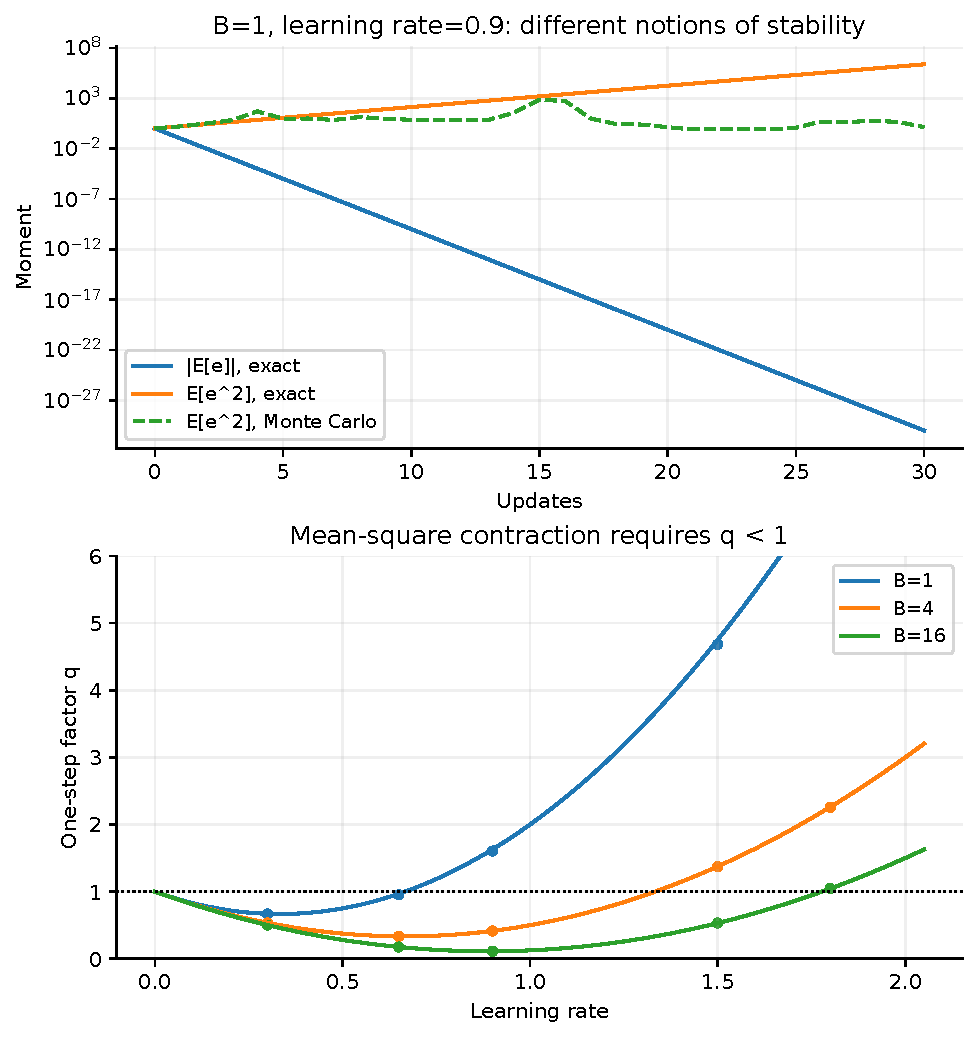
\includegraphics[width=0.85\textwidth]{figures/sgd_stability.pdf}
 \caption{随机回归中均值与均方稳定性的区别，以及单步二阶矩的理论预测与蒙特卡洛核验。解析结果来自本讲的精确矩递推；有限重复次数的蒙特卡洛估计带有抽样误差，特别是在乘性噪声较强时，不能把样本曲线与理论值的偏差直接解释为公式失效。}
 \label{l3:fig-stability}
\end{figure}

\subsection{实验步骤与提交物}

\begin{enumerate}
 \item \textbf{实现并核对梯度。} 设 $a_\star=2$、$s^2=1$、$\tau^2=1/4$。从 $a_0=3$ 出发，每一步重新生成 $x$ 与独立标签噪声。先用自动微分和显式公式 $g=Ae-b$ 在同一个批次上核对一次；损失使用批次平均，不能把求和损失混进学习率比较。
 \item \textbf{观察均值和均方的分离。} 对 $B=1$ 比较 $\eta=0.2$、$0.6$、$1.0$。并行运行多条独立轨迹，记录 $\widehat m_t$、$\widehat q_t$，叠加式\eqref{l3:mean-recurrence}与式\eqref{l3:finite-time-q}。用较短时间窗口观察不稳定组，避免溢出后仍把数值当成有效数据。
 \item \textbf{检查批量相关的边界。} 对 $B=1,4,16$，在各自理论边界 $2B/(B+2)$ 的两侧选择步长。记录均方误差是否收缩，并解释为什么只看平均参数不足以判断稳定。
 \item \textbf{检查线性缩放。} 比较固定学习率和固定 $\eta/B$ 两种设置，同时给出按步数与按已处理样本数排列的曲线。对稳定组报告有限时间理论值与实验值，不要求短轨迹已经到达稳态。
 \item \textbf{形成一页结论。} 每个结论都写明抽样方式、批量、步长、重复次数和预算口径。至少解释一个理论与实验偏差的可能来源，并设计一个能够区分解释的补充检查。
\end{enumerate}

\begin{center}
\small
\begin{tabularx}{\textwidth}{lXXX}
\toprule
应记录的量 & 回答的问题 & 理论对照 & 常见误读\\
\midrule
平均误差 $\widehat m_t$ & 有无平均方向偏差 & 式\eqref{l3:mean-recurrence} & 均值为零即稳定\\
二阶矩 $\widehat q_t$ & 平均风险是否受控 & 式\eqref{l3:finite-time-q} & 单轨迹平滑即可靠\\
样本数 $Bt$ & 数据使用效率 & 固定预算比较 & 每步更快即总训练更快\\
运行时间 & 实际资源效率 & 同设备重复测量 & 把启动开销当算法成本\\
\bottomrule
\end{tabularx}
\end{center}

\subsection{实验读图时的三个检查}

首先检查实现是否真的每步使用新样本。如果反复使用一个固定批次，观察的是另一随机问题。其次检查标签噪声的定义：若把 $\tau$ 当成方差传给要求标准差的生成器，预测的地板会改变。最后检查样本平均与总体期望的区别。稳定组可用更多独立重复缩小误差；不稳定乘性过程的少量极端轨迹可能支配二阶矩，不能通过删除极端值使曲线“符合直觉”。可以另报中位数，但必须保留它与二阶矩是不同统计量这一事实。

\section{习题}
\label{l3:exercises}

\begin{exercise}[抽样协方差]
\label{l3:ex-sampling}
固定 $N=100$ 个样本梯度，总体协方差采用分母 $N$，记为 $\Sigma_N$。分别求 $B=10$ 的有放回和不放回批次均值的协方差。解释为什么一个 epoch 内的随机重排不能在任意当前参数处直接使用条件无偏公式。
\end{exercise}

\begin{exercise}[精确均方递推]
\label{l3:ex-gaussian}
在高斯回归模型中，推导 $\E A_t^2$ 与 $\E b_t^2$。设 $s^2=2$、$B=2$、$\tau^2=1$，求均值稳定和均方稳定的步长区间，并计算 $\eta=0.2$ 时的稳态超额风险。
\end{exercise}

\begin{exercise}[稳态与有限时间]
\label{l3:ex-additive}
对加性噪声模型取 $\lambda=4$、$\sigma_g^2=8$、$B=16$。分别在 $\eta=0.05$ 与 $\eta=0.4$ 时计算稳态损失，并比较近似 $\eta\sigma_g^2/(4B)$ 的误差。说明为什么第二个步长虽稳定，近似却明显较差。
\end{exercise}

\begin{exercise}[非凸保证的适用范围]
\label{l3:ex-nonconvex}
重写式\eqref{l3:conditional-descent}的证明，指出在哪一步使用了条件无偏性、方差上界和光滑性。若希望 $\E\norm{\nabla F(w_R)}^2\leq\epsilon^2$，分别讨论确定性和固定批量随机情形由本讲上界给出的步数阶数。举例说明梯度为零不保证最小值。
\end{exercise}

\begin{exercise}[动量的参数约定]
\label{l3:ex-momentum}
设 $H$ 的特征值为 $1$ 和 $9$。对 Heavy Ball 取 $\beta=1/4$，求全部方向稳定的学习率区间，以及使所有方向同时位于复根区域内部的学习率区间。若改用 $m_t=\beta m_{t-1}+(1-\beta)g_t$，更新 $w_{t+1}=w_t-\alpha m_t$，求与原 Heavy Ball 步长 $\eta$ 等价的 $\alpha$。
\end{exercise}

\begin{exercise}[设计公平的 batch 实验]
\label{l3:ex-batch-design}
同学报告“$B=128$ 的训练损失在 1000 步时比 $B=32$ 低，因此大批量更高效”。给出该结论尚缺少的信息，并设计同时比较样本效率和运行时间效率的方案。在高斯模型中说明为什么即使保持 $\eta/B$，也不能预先保证两组稳态误差完全相同。
\end{exercise}

\section{习题解答要点}
\label{l3:solutions}

\subsection*{习题\ref{l3:ex-sampling}}
有放回协方差是 $\Sigma_N/10$。不放回协方差是
$90/(10\times99)\Sigma_N=\Sigma_N/11$。随机重排的下一批来自剩余样本，而当前参数已受先前样本影响；固定参数时的对称抽样计算，不等于关于训练历史条件化后的无偏性。

\subsection*{习题\ref{l3:ex-gaussian}}
将 $A_t^2$ 展开，$B$ 个同指标项使用 $\E x^4=3s^4$，$B(B-1)$ 个异指标项使用独立性，得到 $s^4(1+2/B)$。$b_t^2$ 的异指标项因标签噪声零均值而消失，得到 $s^2\tau^2/B$。均值稳定要求 $0<\eta<1$，均方稳定要求 $0<\eta<1/2$。取 $\eta=0.2$ 时，
\[
 q_\infty=\frac{0.2}{2[2-0.2\times2\times2]}=\frac1{12}.
\]
超额风险是 $s^2q_\infty/2=1/12$，另外还存在不可约损失 $\tau^2/2$。

\subsection*{习题\ref{l3:ex-additive}}
稳定范围为 $0<\eta<1/2$。精确稳态损失分别为
$0.4/[32(1.8)]=1/144\approx0.006944$ 和
$3.2/[32(0.4)]=1/4$。小步长近似分别为 $0.00625$ 和 $0.05$。第二组的 $\eta\lambda=1.6$ 并不小，分母 $2-\eta\lambda$ 不能用 $2$ 替代。

\subsection*{习题\ref{l3:ex-nonconvex}}
光滑性用于二阶上界；条件无偏性同时用于交叉项和二阶矩分解；方差上界控制剩余噪声项。确定性情形取 $\eta=1/L$，达到梯度平方精度 $\epsilon^2$ 的上界为 $O(\epsilon^{-2})$ 步。固定 $B$ 的一般随机情形，平衡两项后需要 $O(\epsilon^{-4})$ 步。这些阶数将 $L,\Delta,\sigma,B$ 看作固定量。$F(w)=1-\cos w$ 在 $w=\pi$ 处梯度为零但为局部最大值，是直接反例。

\subsection*{习题\ref{l3:ex-momentum}}
稳定区间为 $0<\eta<2(1+1/4)/9=5/18$。复根要求对 $\lambda=1$ 有 $\eta>1/4$，对 $\lambda=9$ 有 $\eta<(3/2)^2/9=1/4$，严格区间为空；在 $\eta=1/4$ 时两个端点恰好成为重根，这也是本例经典最优二次参数。若两种动量均从零开始，$m_t=(1-\beta)v_t$，所以 $\alpha=\eta/(1-\beta)=4\eta/3$。

\subsection*{习题\ref{l3:ex-batch-design}}
原比较使用了四倍样本，且尚未说明设备、吞吐、学习率、初始化、目标精度和重复次数。应固定模型、数据及随机种子集合，分别画损失对已处理样本数和损失对运行时间的曲线，并比较到达同一阈值的成本。高斯模型的精确地板除 $\eta/B$ 外，还含 $2-\eta s^2(1+2/B)$；保持比值不保持分母。可以在足够小的步长下提出近似相同的预测，再用实验检查近似误差。

\begin{coursebox}{离开本讲时应保留的判断顺序}
先定义目标与抽样，再检查均值和二阶矩，随后说明收敛指标与计算预算。对动量，先写完整状态递推和学习率约定，再判断稳定区域。进入深度网络后，可以使用这些小模型形成可检验的预测，但需要重新核对其假设，不能把模型中的充分条件或近似规律直接称为所有网络的训练定律。
\end{coursebox}
